\newpage
\def\thoigian{90}%--Thời gian
\de{Đề số 2}{Chương IX. Phương pháp tọa độ trong mặt phẳng}


\begin{center}
	\textbf{PHẦN 1-CÂU TRẮC NGHIỆM BỐN PHƯƠNG ÁN}
\end{center}
\Opensolutionfile{ans}[ans/ans-TN-ONTAPCHUONG-DE1]

%Câu 1
\begin{ex}%[Dự án D đợt 3, BCTuan]%[0H9N1-1]
	Trong mặt phẳng $Oxy$, cho véc-tơ $\overrightarrow{OA} =-3\overrightarrow{i}+7\overrightarrow{j}$. Tọa độ của điểm $A$ là
	\choice
	{$A(7;-3)$}
	{$A(-7; 3)$}
	{\True $A(-3; 7)$}
	{$A(3;-7)$}
	\loigiai{
		Ta có $\overrightarrow{OA} =-3\overrightarrow{i}+7\overrightarrow{j}\Rightarrow A(-3; 7)$.
	}
\end{ex}
\begin{ex}%[Dự án D đợt 3, BCTuan]%[0H9H1-3] 
	Trong mặt phẳng $Oxy$, cho $A(2;4)$, $B(-1;-4)$. Tìm tọa độ điểm $D$ để tứ giác $OABD$ là hình bình hành.
	\choice
	{$D(3;-8)$}
	{\True $D(-3;-8)$}
	{$D(3;8)$}
	{$D(-3;8)$}
	\loigiai{
		Gọi điểm $D(x;y)$, ta có $\overrightarrow{AB}=(-3;-8)$, $\overrightarrow{OD}=(x;y)$.\\
		Vì $OABD$ là hình bình hành nên $\overrightarrow{AB}=\overrightarrow{OD} \Leftrightarrow \heva{&x=-3\\&y=-8}$.\\
		Vậy tọa độ điểm $D(-3;-8)$.
	}
\end{ex}
\begin{ex}%[Dự án D đợt 3, BCTuan]%[0H9N1-3]
	Trong mặt phẳng $Oxy$, cho ba điểm không thẳng hàng $A(3;-1)$, $B(2; 10)$, $C(4;-2)$. Tính tọa độ trọng tâm $G$ của tam giác $ABC$.
	\choice
	{$G\left(-3;-\dfrac{7}{3}\right)$}
	{$G\left(-3; \dfrac{7}{3}\right)$}
	{$G(-3;3)$}
	{\True $G\left(3;\dfrac{7}{3}\right)$}
	\loigiai{
		Vì $G$ là trọng tâm của $\triangle ABC$ nên $\heva{&x_G = \dfrac{x_A+x_B+x_C}{3}\\&y_G = \dfrac{y_A+y_B+y_C}{3}} \Rightarrow \heva{&x_G = \dfrac{3+2+4}{3} = 3\\&y_G = \dfrac{-1+10+(-2)}{3} = \dfrac{7}{3}} \Rightarrow G\left(3;\dfrac{7}{3}\right)$.
	}
\end{ex}
\begin{ex}%[Dự án D đợt 3, BCTuan]%[0H9N3-1]
	Trong mặt phẳng tọa độ $Oxy$, cho đường thẳng $\Delta\colon x-2y+3=0$. Véc-tơ nào sau đây \textbf{không} là véc-tơ chỉ phương của $\Delta$?
	\choice
	{\True $\overrightarrow{u}_1=(4;-2)$}
	{$\overrightarrow{u}_2=(-2;-1)$}
	{$\overrightarrow{u}_3=(2;1)$}
	{$\overrightarrow{u}_4=(4;2)$}
	\loigiai{
		Đường thẳng $\Delta $ có véc-tơ pháp tuyến $\overrightarrow{n}=(1;-2)$ nên suy ra véc-tơ chỉ phương của nó là $\overrightarrow{u}=(2;1)$.\\ 
		Trong bốn phương án ta thấy có $(4;-2)$ không cùng phương với $\overrightarrow{u}=(2;1)$.
	}	
\end{ex}
\begin{ex}%[Dự án D đợt 3, BCTuan]%[0H9H3-2]
	Trong mặt phẳng $Oxy$, đường thẳng $\Delta$ đi qua điểm $H(3; -4)$ và song song với đường thẳng $d\colon x-2y+7=0$ có phương trình là
	\choice
	{$\Delta\colon x-2y+11 = 0$}
	{$\Delta\colon 2x+y+2 = 0$}
	{\True $\Delta\colon x-2y-11 = 0$}
	{$\Delta\colon 2x+y-2 = 0$}
	\loigiai{
		Ta có $\Delta \parallel d$ nên $\Delta \colon x-2y+m =0$ ($m\ne 7$).\\
		Mà $\Delta$ đi qua $H(3; -4)$ nên $3-2\cdot (-4) +m=0$ hay $m=-11$.\\
		Vậy phương trình $\Delta \colon x-2y-11 = 0$.
	}
\end{ex}
\begin{ex}%[Dự án D đợt 3, BCTuan]%[0H9H3-3]
	Trong mặt phẳng $Oxy$, cho đường thẳng $d_1\colon 2x+3y+15=0$ và $d_2\colon 3x+2y-3=0$. Khẳng định nào sau đây là đúng?
	\choice
	{\True $d_1$ và $d_2$ cắt nhau và không vuông góc với nhau}
	{$d_1$ và $d_2$ song song với nhau}
	{$d_1$ và $d_2$ trùng nhau}
	{$d_1$ và $d_2$ vuông góc với nhau}
	\loigiai 
	{
		Xét hệ phương trình 
		$\heva{& 2x+3y=-15 \\ & 3x+2y=3}\Leftrightarrow\heva{& x=\dfrac{39}{5}\\ & y=-\dfrac{51}{5}.}$\\
		Hệ phương trình có một nghiệm duy nhất nên $d_1$ cắt $d_2$ ($1$).\\
		Mặt khác $\overrightarrow{n}_1\cdot\overrightarrow{n}_2=2\cdot 3+3\cdot 2=12\ne 0$ nên $d_1$ không vuông góc $d_2$ $(2)$.\\
		Từ $(1)$ và $(2)$ ta suy ra $d_1$ và $d_2$ cắt nhau và không vuông góc với nhau.
	}
\end{ex}
\begin{ex}%[Dự án D đợt 3, BCTuan]%[0H9N4-2]
	Trong mặt phẳng $Oxy$, đường tròn $(C)$ có tâm $I(3;1)$ và có đường kính bằng $4$ có phương trình là
	\choice
	{\True $(x-3)^2+(y-1)^2=4$}
	{$(x+3)^2+(y+1)^2=4$}
	{$(x+3)^2+(y+1)^2=2$}
	{$(x-3)^2+(y-1)^2=16$}
	\loigiai{
		Bán kính của đường tròn $(C)$ bằng $\dfrac{4}{2}=2$. \\
		Phương trình đường tròn $(C)$ tâm $I(3;1)$ bán kính bằng $2$ là $$(x-3)^2+(y-1)^2=4.$$
	}
\end{ex}
\begin{ex}%[Dự án D đợt 3, BCTuan]%[0H9H4-2]
	Trong mặt phẳng tọa độ $Oxy$, phương trình đường tròn $(C)$ có tâm $I(1;-2)$ và tiếp xúc với đường thẳng $2x+y+5=0$ là
	\choice
	{$(x-1)^2+(y+2)^2=1$}
	{\True $(x-1)^2+(y+2)^2=5$}
	{$(x-1)^2+(y+2)^2=25$}
	{$(x+1)^2+(y-2)^2=5$}
	\loigiai{
		Ta có bán kính $R=\mathrm{d}(I,\Delta)=\dfrac{|2\cdot 1-2+5}{\sqrt{2^2+1^2}}=\sqrt{5}$.\\ 
		Do đó phương trình $(C)$ là $(x-1)^2+(y+2)^2=5$.
	}
\end{ex}
\begin{ex}%[Dự án D đợt 3, BCTuan]%[0H9N4-4]
	Trong mặt phẳng $Oxy$, điểm $A(1;1)$ nằm trên đường tròn nào sau đây?
	\choice
	{\True $(x-4)^2+y^2=10$}
	{$(x-1)^2+(y-1)^2=4$}
	{$(x-2)^2+y^2=5$}
	{$(x+1)^2+(y-1)^2=3$}
	\loigiai{
		Ta có $(1-4)^2+1^2=10$ nên điểm $A(1;1)$ nằm trên đường tròn $(x-4)^2+y^2=10$.
	}
\end{ex}
\begin{ex}%[Dự án D đợt 3, BCTuan]%[0H9N5-4]
	Trong mặt phẳng $Oxy$, độ dài trục ảo của hypebol $(H) \colon \dfrac{x^2}{16}-\dfrac{y^2}{25}=1$ bằng 
	\choice
	{$10$}
	{\True $8$}
	{$32$}
	{$50$}
	\loigiai{
		Ta có $b^2 = 25$ nên $b = 5$ (do $b>0$). \\
		Độ dài trục ảo là $2b = 10$. 
	}
\end{ex}
\begin{ex}%[Dự án D đợt 3, BCTuan]%[0H9H5-7]
	Trong mặt phẳng $Oxy$, cho phương trình chính tắc parabol là $y^2=4x$. Xác định tiêu điểm của parabol trên.
	\choice
	{$(2;0)$}
	{\True $(1;0)$}
	{$(4;0)$}
	{$(-2;0)$}
	\loigiai{
		Ta có $2p=4\Leftrightarrow p=2$.\\
		Suy ra tiêu điểm của parabol là $(1;0)$.
	}
\end{ex}
\begin{ex}%[Dự án D đợt 3, BCTuan]%[0H9H5-1]
	Trong mặt phẳng $Oxy$, cho elip có phương trình chính tắc $\dfrac{x^2}{25}+\dfrac{y^2}{16}=1$. Xác định tiêu cự của elip.
	\choice
	{$3$}
	{$8$}
	{$10$}
	{\True $6$}
	\loigiai{
		Xét phương trình elip $\dfrac{x^2}{25}+\dfrac{y^2}{16}=1$.\\
		Ta có $\heva{&a^2=25\\&b^2=16} \Rightarrow c^2=a^2-b^2=25-16=9 \Rightarrow c=3$.\\
		Tiêu cự của elip là $2c=6$.
	}
\end{ex}
\Closesolutionfile{ans}
%\begin{center}
%	\textbf{ĐÁP ÁN}
%	\inputansbox{10}{ans/ans}	
%\end{center}



\begin{center}
	\textbf{PHẦN 2-CÂU TRẮC NGHIỆM ĐÚNG SAI}
\end{center}
\setcounter{ex}{0}% Reset lại số đếm câu hỏi
\Opensolutionfile{ans}[ans/answer-DS-ONTAPCHUONG-DE1]
\begin{ex}%[Dự án D đợt 3, BCTuan]%[0H9V3-5]
	Trong mặt phẳng $Oxy$, cho đường thẳng $\Delta \colon 3x-4y+10=0$.
	\choiceTF
	{\True Khoảng cách từ gốc tọa độ $O$ đến đường thẳng $\Delta$ bằng $2$}
	{Đường thẳng $\Delta$ đi qua điểm $M(1;2)$}
	{Gọi $\alpha$ là góc giữa đường thẳng $\Delta$ và đường thẳng $d\colon x+y-1=0$. Khi đó $\tan\alpha=\dfrac{1}{7}$}
	{\True Một véc-tơ pháp tuyến của đường thẳng $\Delta$ là $\overrightarrow{n}=(3;-4)$}
	\loigiai{
		\begin{itemchoice}
			\itemch Ta có $\mathrm{d}\left(O,\Delta\right)=\dfrac{|3\cdot 0-4\cdot 0+10|}{\sqrt{3^2+(-4)^2}}=2$.
			\itemch Thay tọa độ của $M(1;2)$ vào phương trình của $\Delta$ ta được $3-8+10=0$, vô lí.\\
			Vậy $M(1;2)$ không thuộc $\Delta$.
			\itemch Ta có $\cos\alpha=\dfrac{|3\cdot 1-4\cdot 1|}{\sqrt{3^2+(-4)^2}\cdot \sqrt{1^2+1^2}}=\dfrac{1}{5\sqrt{2}}$.\\
			Ta có $1+\tan^2\alpha =\dfrac{1}{\cos^2\alpha}=50\Rightarrow\tan\alpha =7$.
			\itemch Một véc-tơ pháp tuyến của đường thẳng $\Delta$ là $\overrightarrow{n}=(3;-4)$.
		\end{itemchoice}
	}
\end{ex}
\begin{ex}%[Dự án D đợt 3, BCTuan]%[0H9V4-7]
	\immini{Trong một trò chơi điện tử, màn hình của người chơi được xem là một hệ trục tọa độ $Oxy$ với điểm $O$ nằm ở góc trái màn hình (tham khảo hình vẽ). Nòng súng của người chơi ở vị trí có tọa độ $A(2;1)$, đang ngắm bắn các mục tiêu thuộc đường tròn $(x-10)^2+(y-5)^2=4$. Nếu người chơi bắn trúng hai mục tiêu $B$, $C$ cùng lúc (dây cung $BC$ của đường tròn) thì số điểm của người chơi được tính bằng cách lấy phần nguyên của độ dài $BC$ rồi nhân với $10$.}
	{\begin{tikzpicture}[line join = round, line cap=round,>=stealth,font=\footnotesize,scale=0.71]
			\clip (-1,-1) rectangle (11,7);
			\tikzset{nguoilinh/.pic={ 
					\draw[fill=black] (8.2, 17.8)--(8.1, 17.9)--(8.1, 18.2)--(8, 18.4)--(7.9, 19)..controls+(63.43: 0.22)and+(153.43: 0.22)..(8.3,19.2)--(8.4, 19.5)..controls+(161.57: 0.32)and+(-90: 0.1)..(8.1,19.8)..controls+(135: 0.14)and+(-135: 0.14)..(8.1,20.2)..controls+(45: 0.14)and+(135: 0.14)..(8.5,20.4)..controls+(26.57: 0.22)and+(135: 0.14)..(8.9,20.4)..controls+(0: 0.2)and+(90: 0.1)..(9.3,20.2)..controls+(0: 0)and+(0: 0.1)..(9.3,20.1)..controls+(-90: 0.1)and+(90: 0.1)..(9.3,19.9)..controls+(0: 0)and+(180: 0.1)..(9.4,19.9)..controls+(-90: 0.1)and+(0: 0)..(9.4,19.7)--(9.3, 19.6)..controls+(-135: 0.14)and+(90: 0.1)..(9.2,19.3)..controls+(0: 0)and+(180: 0.1)..(9.4,19.2)..controls+(90: 0.1)and+(180: 0.1)..(9.6,19.4)..controls+(135: 0.14)and+(-90: 0.1)..(9.6,19.6)--(9.7, 19.5)--(9.8, 19.6)..controls+(90: 0.1)and+(180: 0.1)..(9.9,19.8)..controls+(0: 0.1)and+(90: 0.1)..(10.1,19.7)..controls+(0: 0.1)and+(-135: 0.14)..(10.4,19.7)..controls+(90: 0.3)and+(-161.57: 0.32)..(11,20.1)..controls+(45: 0.14)and+(180: 0.1)..(11.3,20.3)..controls+(-90: 0.2)and+(90: 0.1)..(11.2,19.9)..controls+(-161.57: 0.32)and+(26.57: 0.22)..(10.8,19.6)--(10.8, 19.4)--(10.6, 19.2)--(10.7, 
					19)--(10.8, 18.9)--(10.7, 18.7)--(10.5, 18.7)--(10.5, 18.5)--(10.3, 18.2)--(10, 18.4)--(9.7, 18.4)--(9.6, 18.2)--(9.7, 17.9)..controls+(180: 0.2)and+(90: 0.1)..(9.5,17.7)--(9.6, 17.5)..controls+(-45: 0.42)and+(123.69: 0.36)..(10.4,16.7)..controls+(0: 0.1)and+(104.04: 0.41)..(10.6,16.4)..controls+(-135: 0.14)and+(116.57: 0.22)..(10.5,15.9)--(10.4, 15.7)..controls+(-135: 0.14)and+(90: 0.1)..(10.4,15.4)..controls+(-45: 0.14)and+(180: 0.2)..(10.9,15.2)--(10.9, 15)--(10.7, 14.9)--(10.2, 15)--(9.9, 15)--(9.7, 15.2)--(10, 15.5)..controls+(135: 0.14)and+(-90: 0.2)..(9.8,16)..controls+(26.57: 0.22)and+(-135: 0.14)..(10,16.3)..controls+(153.43: 0.45)and+(-45: 0.28)..(9.2,16.9)..controls+(135: 0.14)and+(0: 0.1)..(8.9,16.9)..controls+(-135: 0.28)and+(90: 0.3)..(8.7,16.2)..controls+(-116.57: 0.22)and+(18.43: 0.32)..(8.1,15.8)--(8, 15.7)--(7.8, 15.7)--(7.8, 15.6)--(7.9, 15.4)..controls+(0: 0.3)and+(180: 0.1)..(8.4,15.3)..controls+(-90: 0.1)and+(26.57: 0.22)..(8.2,15)..controls+(153.43: 0.22)and+(-26.57: 0.22)..(7.7,15.2)..controls+(-90: 0.1)and+(0: 0.1)..(7.5,15.1)..controls+(180: 0.2)and+(-45: 0.14)..(7.1,15.3)..controls+(0: 0.1)and+(180: 0.3)..(7.4,15.5)..controls+(180: 0.1)and+(-135: 0.14)..(7.4,15.7)--(7.5, 15.8)--(7.6, 16)..controls+(180: 0.1)and+(-90: 0.2)..(7.5,16.2)--(7.8, 16.3)--(8.1, 16.5)--(8.1, 16.8)--(8.2, 17.1)--(8.2, 17.3)--(8.1, 17.5)--(8.2, 17.6)--cycle;
					\path[fill=black!40,opacity=0.4,name path=circle] (22,25) circle(2cm); 
					\path[draw,dashed,name path=line] (11.3,20.3)coordinate (A)--(26.3,28.3) ; 
					\path [draw,name intersections={of=line and circle, by={C,B}}];
					\draw[fill=white] (10.1, 18.8) -- (9.9, 18.9) -- 
					(9.9, 19.0) -- (10.1, 19.1) -- (10.2, 19.1) -- (10.2, 18.9) -- cycle;
			}}
			%\draw ;
			\path(-2.5,-6)pic[scale=0.285]{nguoilinh};
			\fill 
			(A) circle(1.5pt)node[above]{$A$}
			(B) circle(1.5pt)node[above left]{$B$}
			(C) circle(1.5pt)node[above]{$C$}
			(0,0) circle(1.5pt)node[below]{$O$}
			;
			\draw[->] (0,0)--(10,0) node[below]{$x$};	
			\draw[->] (0,0)--(0,6) node[left]{$y$};	
	\end{tikzpicture}}
	\choiceTF
	{\True Đường tròn chứa mục tiêu có tâm $I(10;5)$, bán kính bằng $2$}
	{Nếu nòng súng người chơi nhắm theo hướng véc-tơ $\vec{u}=(2;3)$ thì viên đạn sẽ bay theo đường thẳng có phương trình $\heva{&x=2+3t\\&y=1-2t}$ ($t$ là tham số)}
	{\True Nếu người chơi bắn viên đạn theo hướng véc-tơ $\vec{v}=(2;1)$ thì điểm số thu được là tối đa}
	{Nếu người chơi bắn trúng mục tiêu có tọa độ $(10;3)$ thì điểm số thu được bằng $10$}
	\loigiai{\begin{itemchoice}
			\itemch Đường tròn chứa mục tiêu có tâm $I(10;5)$, bán kính bằng $R=2$.
			\itemch Viên đạn bay theo đường thẳng đi qua $A(2;1)$ và có véc-tơ chỉ phương $\vec{u}=(2;3)$ nên có phương trình là $\heva{&x=2+2t\\&y=1+3t.}$
			\itemch Nếu người chơi bắn viên đạn theo hướng véc-tơ $\vec{v}=(2;1)$ thì đường bay của viên đạn có phương trình là $d\colon\heva{&x=2+2t\\&y=1+t.}$\\
			Nhận thấy khi đó tọa độ của tâm $I$ thỏa mãn phương trình đường thẳng $d$. Suy ra viên đạn đi qua tâm $I$, vậy $BC$ có độ dài lớn nhất nên điểm số thu được là tối đa.
			\itemch \immini{Nếu người chơi bắn trúng mục tiêu là $M(10;3)$ thì viên đạn sẽ bay theo đường thẳng đi qua $A(2;1)$ và có véc-tơ chỉ phương là $\vec{AM}=(8;2)$ nên có phương trình tổng quát là $x-4y+2=0$.\\
				Gọi $H$ là hình chiếu của $I$ lên $AM$, ta có
				\[IH=\mathrm{d}(I,AM)=\dfrac{|10-4\cdot5+2|}{\sqrt{1+16}}=\dfrac{8\sqrt{17}}{17}.\]
				Gọi $N$ là mục tiêu còn lại khi đã bắn trúng $M$, ta có
				\[MN=2\sqrt{R^2-IH^2}=\dfrac{4\sqrt{17}}{17}\approx0{,}97.\]
				Khi đó số điểm được nhận của người chơi là $T=0\cdot10=0$\, (điểm).}
			{\begin{tikzpicture}[>=stealth,line join=round,line cap=round,font=\footnotesize,scale=0.5]
					\path
					(0,0) coordinate (I)++(-90:3)coordinate (M)
					(-7,-6) coordinate (A)
					($(M)!(I)!(A)$) coordinate (H)
					($(M)!2!(H)$) coordinate (N)
					;
					\draw (I) circle (3) (A)--(N)--(I)--(H);
					\foreach \p / \r in {A/135,M/-45,N/-45,I/45,H/-45}
					\fill (\p) circle (1.2pt) node[shift={(\r:3mm)}]{$\p$};
					\pic[draw,angle radius=1.2mm,angle eccentricity=1.5] {right angle = I--H--N};
			\end{tikzpicture}}
	\end{itemchoice}}
\end{ex}
\Closesolutionfile{ans}
%\inputansbox[2]{2}{ans/answer.tex}



\begin{center}
\textbf{PHẦN 3-CÂU TRẮC NGHIỆM TRẢ LỜI NGẮN}
\end{center}
\setcounter{ex}{0}
\Opensolutionfile{ans}[ans-KQ-ONTAPCHUONG-DE1]

\begin{ex}%[Dự án D đợt 3, BCTuan]%[0H9V4-7]
	Trong công viên có một cái ghế được tạo hình là một đường thẳng $\Delta$ đặt trong một khung tròn $(C)$ như hình minh họa. Nếu đặt trong mặt phẳng $Oxy$ thích hợp, cho đường tròn $(C)$ có tâm $I(3;2)$ và phương trình đường thẳng $\Delta\colon x-y+1=0$. Biết $\Delta$ cắt đường tròn $(C)$ tại hai điểm $A$ và $B$ sao cho tam giác $IAB$ vuông. Tính bán kính của đường tròn $(C)$.
	\begin{center}
		\begin{tikzpicture}[line join = round, line cap=round,>=stealth,font=\footnotesize,scale=.7]
			\path[draw=black!20,line width=10pt,name path=circle] (0,0) circle(2 cm); 
			\path[draw=brown,line width=4pt,name path=line](-165:2.5)--(-15:2.5); 
			\path [name intersections={of=line and circle, by={A,B}}];
			\draw[line width=4pt,brown] 
			(A)--(-135:4cm)
			(B)--(-45:4cm)
			;
		\end{tikzpicture}
		\begin{tikzpicture}[scale=.7, font=\footnotesize, line join=round, line cap=round, >=stealth]
			\path 
			(-45:2) coordinate (B)
			(-135:2) coordinate (A)
			(0,0) coordinate (I)
			;
			\draw (I) circle (2cm) (A)--(I)--(B)
			($(A)!2!(B)$)--($(B)!2!(A)$)
			;
			\fill ($(B)!1.5!(A)$)+(90:.2) node{$\Delta$};
			\foreach \d/\g in {A/-135, B/-45, I/90}
			\fill (\d) circle(1pt)+(\g:.3) node{$\d$};
			\draw pic[draw,angle radius=1.5mm] {right angle = A--I--B};
		\end{tikzpicture}
	\end{center}
	\par
	\shortans[oly]{2}
	\loigiai{
		\begin{center}
			\begin{tikzpicture}[scale=.7, font=\footnotesize, line join=round, line cap=round, >=stealth]
				\path 
				(-45:2) coordinate (B)
				(-135:2) coordinate (A)
				(0,0) coordinate (I)
				($(A)!.5!(B)$) coordinate (M)
				;
				\draw (I) circle (2cm) (A)--(I)--(B) (I)--(M)
				($(A)!2!(B)$)--($(B)!2!(A)$)
				;
				\fill ($(B)!1.5!(A)$)+(90:.2) node{$\Delta$};
				\foreach \d/\g in {A/-135, B/-45, I/90,M/-90}
				\fill (\d) circle(1pt)+(\g:.3) node{$\d$};
				\draw pic[draw,angle radius=1.5mm] {right angle = A--I--B};
				\draw pic[draw,angle radius=1.5mm] {right angle = B--M--I};
			\end{tikzpicture}
		\end{center}
		Theo bài ra ta có $\triangle AIM$ vuông cân tại $I$.
		Gọi $M$ là trung điểm của $AB$, suy ra $IM\perp AB$ và $IM=\dfrac{AB}{2}=MB$.\\
		Do đó $IM$ là khoảng cách từ $I$ đến $\Delta$.\\
		Ta có $IM=\mathrm{d}(I,\Delta)=\dfrac{|3-2+1|}{\sqrt{1^2+(-1)^2}}=\sqrt{2}$, suy ra $MB=\sqrt{2}$.\\
		Trong $\triangle IMB$ vuông cân tại $M$, ta có $IB=\sqrt{IM^2+MB^2}=\sqrt{2+2}=2$.\\
		Vậy bán kính đường tròn $(C)$ là $R=IB=2$.
	}
\end{ex}

\begin{ex}%[Dự án D đợt 3, BCTuan]%[0H9H4-3]
	Trong mặt phẳng $Oxy$, cho đường tròn $(C)\colon (x-2)^2+(y+3)^2= 10$. Tiếp tuyến của đường tròn $(C)$ tại điểm $M(5;-2)$ có phương trình là $ax+by-13=0$. Khi đó $3a-4b$ bằng bao nhiêu?
	\shortans[oly]{$5$}
	\loigiai{
		Đường tròn có tâm $I(2;-3)$, bán kính $R=\sqrt{10}$.\\
		Tiếp tuyến tại điểm $M(5;-2)$ vuông góc với bán kính $IM$ nên có véc-tơ pháp tuyến là 
		$$\overrightarrow{IM}=\overrightarrow{n}=(5-2;\-2-(-3))=(3;1).$$
		Phương trình tiếp tuyến tại $M$ có dạng 
		$$3(x-5)+1(y+2)=0 \Rightarrow 3x+y-13=0.$$
		So sánh với dạng $a x+b y-13=0$ ta suy ra 
		$a=3$, $b=1$.\\
		Vậy $3a-4b=3\cdot 3-4\cdot 1=9-4=5$.
	}
\end{ex}
\begin{ex}%[Dự án D đợt 3, BCTuan]%[0H9V5-3]
	Trong mặt phẳng tọa độ $Oxy$, cho elip có hai tiêu điểm lần lượt là $F_1$, $F_2$. Từ các điểm $F_1$, $F_2$ lần lượt kẻ các đường thẳng song song với $Oy$, cắt elip tại các điểm $M$, $N$, $P$, $Q$. Biết bốn điểm $M$, $N$, $P$, $Q$ là bốn đỉnh của một hình vuông. Tính tâm sai $e$ của elip là tỷ số $\dfrac{c}{a}$ của nó (kết quả làm tròn đến hàng phần trăm).
	\shortans[oly]{$0{,}62$}
	\loigiai{
	\begin{center}
	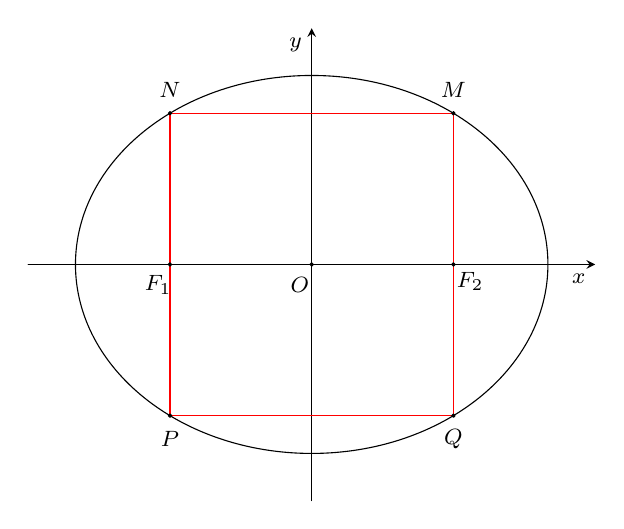
\begin{tikzpicture}[scale=.6,>=stealth, font=\footnotesize, line join=round, line cap=round]
\path (0,0) coordinate (O) (3,0) coordinate (F_2) (-3,0) coordinate (F_1) (-3,3.2) coordinate (N) (-3,-3.2) coordinate (P) (3,3.2) coordinate (M) (3,-3.2) coordinate (Q); 
	\draw[->] (-6,0)--(6,0) node[below left] {$x$};
	\draw[->] (0,-5)--(0,5)  node[below left] {$y$};
	\draw (O) ellipse (5cm and 4cm);
\draw[red] (M)--(N)--(P)--(Q)--cycle;
\foreach \d/\g in {O/-120,F_1/-120,F_2/-45, M/90,N/90,P/-90,Q/-90}
\draw[fill=black] (\d) circle (1pt) +(\g:5mm) node{$\d$}; 
\end{tikzpicture}		
	\end{center}
		Giả sử elip có phương trình $\dfrac{x^2}{a^2}+\dfrac{y^2}{b^2}=1\ (a>b>0)$ và tọa độ hai tiêu điểm $F_1(-c;0)$, $F_2(c;0)$\ $(c^2=a^2-b^2)$.\\
		Ta giả sử điểm $M$ ở góc phần tư thứ I, vì $MNPQ$ là hình vuông nên $M(c;c)$.\\ 
		Thay vào phương trình elip ta có
		$$\dfrac{c^2}{a^2}+\dfrac{c^2}{b^2}=1\Leftrightarrow e^2+\dfrac{c^2}{a^2-c^2}=1\Leftrightarrow e^2+\dfrac{e^2}{1-e^2}=1.$$
		Giải phương trình trên ta có $e^2=\dfrac{3-\sqrt{5}}{2}$. Vậy $e=\dfrac{\sqrt{5}-1}{2}\approx 0{,}62$.
	}
\end{ex}
\begin{ex}%[Dự án D đợt 3, BCTuan]%[0H9V3-8]
	Một khuôn viên được quy hoạch dưới dạng tam giác, với ba cột mốc được đặt tại các vị trí $A(0;0)$, $B(4;5)$ và $C(6;-1)$ (tọa độ theo hệ trục $Oxy$, đơn vị mét). Một robot giao thư bắt đầu từ điểm $N(5;3)$. Robot được lập trình để di chuyển đến một điểm $P$ nằm trên đường thẳng $AC$ để thực hiện trung chuyển, sau đó tiếp tục di chuyển đến trung tâm điều phối được đặt tại trọng tâm $G$ của tam giác $ABC$. Robot cần chọn vị trí $P \in AC$ sao cho tổng quãng đường di chuyển từ $N$ đến $P$, rồi từ $P$ đến trọng tâm $G$ là ngắn nhất. Hãy tính quãng đường ngắn nhất theo lộ trình đó (Kết quả làm tròn đến hàng phần mười).
	\begin{center}
		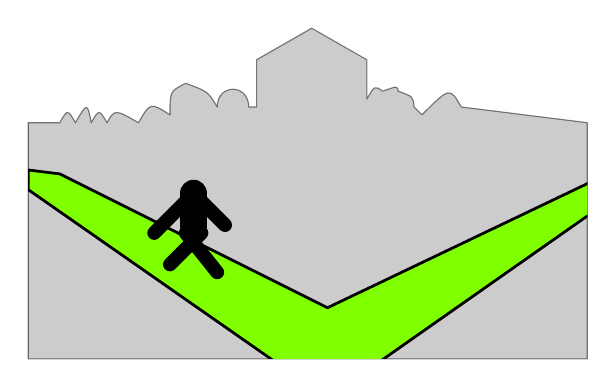
\begin{tikzpicture}[line join = round, line cap=round,>=stealth,font=\footnotesize,scale=1]
			\draw[fill=black!40,opacity=0.5] (0,0)--(0,3)--(0.4,3) 
			.. controls +(60:0.2) .. (0.6,3) .. controls +(60:0.3) .. (0.8,3)
			.. controls +(60:0.2) .. (1,3)
			.. controls +(60:0.2) .. (1.4,3)
			.. controls +(60:0.3) .. (1.8,3.1)
			.. controls +(90:0.3) .. (2,3.5)
			.. controls +(-20:0.3) .. (2.4,3.2)
			.. controls +(90:0.3) and +(90:0.3) .. (2.8,3.2)--(2.9,3.2)--(2.9,3.8)--(3.6,4.2)--(4.3,3.8)--(4.3,3.3)
			.. controls +(60:0.2) .. (4.5,3.4).. controls +(20:0.2) .. (4.7,3.4)
			.. controls +(-20:0.2) .. (4.9,3.2)--(5,3.1).. controls +(45:0.5) .. (5.5,3.2)--(7.1,3)--(7.1,0)--cycle
			;
			
			\clip (0,0)--(0,3)--(7.1,3)--(7.1,0)--cycle;
			\draw[fill=green!50!yellow,line width=1pt] (0,2.15) -- (0,2.40) -- (0.4,2.35) -- (3.8,0.65) -- (7.15,2.25) -- (7.15,1.85) -- (3.8,-0.5) -- (0,2.15);
			\draw[line width=10pt] (2.1,2.1) -- (2.1,1.7);
			\draw[line width=5pt] (2.1,2.1)--(1.6,1.6) (2.1,2.1)--(2.5,1.7)(2,1.6)--(2.4,1.1)(2.2,1.6)--(1.8,1.2);
		\end{tikzpicture}
		\begin{tikzpicture}[scale=.8,>=stealth, font=\footnotesize, line join=round, line cap=round]
			\tikzset{every node/.style={scale=1}}
			\path
			(0,0) coordinate (A) 
			(4,5) coordinate (B)
			(6,-1) coordinate (C)
			(5,3) coordinate (N)
			($(A)!.55!(C)$) coordinate (P)
			($(A)!.5!(B)$) coordinate (C')
			($(A)!.5!(C)$) coordinate (B')
			(intersection of B--B' and C--C') coordinate (G)
			;
			\draw[->] (-1,0)--(7,0) node[below left] {$x$};
			\draw[->] (0,-2)--(0,6)  node[below left] {$y$};
			\fill 
			(4,0)node[below]{$4$} circle(1pt)
			(0,5)node[left]{$5$} circle(1pt)
			(6,0)node[above]{$6$} circle(1pt)
			(0,-1)node[left]{$-1$} circle(1pt)
			(5,0)node[below]{$5$} circle(1pt)
			(0,3)node[left]{$3$} circle(1pt)
			;
			\draw[dashed] (6,0)|-(0,-1) (5,0)|-(0,3) (4,0)|-(0,5); 
			\draw
			(A)--(B)--(C)--cycle (G)--(P)--(N) ;
			\foreach \x/\g in
			{A/210,B/90,C/-90,P/-90,G/180,N/90}
			\fill[black](\x) circle (1pt)
			($(\x)+(\g:3mm)$) node{$\x$};
		\end{tikzpicture}
	\end{center}
	\shortans{$5{,}8$}
	\loigiai{
		\begin{center}
			\begin{tikzpicture}[scale=.8,>=stealth, font=\footnotesize, line join=round, line cap=round]
				\tikzset{every node/.style={scale=1}}
				\path
				(0,0) coordinate (A) 
				(4,5) coordinate (B)
				(6,-1) coordinate (C)
				(5,3) coordinate (N)
				($(A)!.5!(B)$) coordinate (C')
				($(A)!.5!(C)$) coordinate (B')
				(intersection of B--B' and C--C') coordinate (G)
				(162/37,-27/37) coordinate (K)
				($(N)!2!(K)$) coordinate (N')
				(intersection of G--N' and C--A) coordinate (P)
				;
				\draw[->] (-1,0)--(7,0) node[below left] {$x$};
				\draw[->] (0,-5)--(0,6)  node[below left] {$y$};
				\fill 
				(4,0)node[below]{$4$} circle(1pt)
				(0,5)node[left]{$5$} circle(1pt)
				(6,0)node[above]{$6$} circle(1pt)
				(0,-1)node[left]{$-1$} circle(1pt)
				(5,0)node[below]{$5$} circle(1pt)
				(0,3)node[left]{$3$} circle(1pt)
				;
				\draw[dashed] (6,0)|-(0,-1) (5,0)|-(0,3) (4,0)|-(0,5); 
				\draw
				(A)--(B)--(C)--cycle (G)--(N')--(N)--(P) ;
				\foreach \x/\g in
				{A/210,B/90,C/-90,P/-120,G/180,N/90,K/40,N'/0}
				\fill[black](\x) circle (1pt)
				($(\x)+(\g:3mm)$) node{$\x$};
			\end{tikzpicture}
		\end{center}
		Phương trình đường thẳng $AC$ qua $A(0;0)$ và nhận  $\overrightarrow{AC}=(6;-1)$ làm véc-tơ chỉ phương có phương trình tham số là $\heva{&x=6t\\&y=-t.}$\\
		Ta có $G$ là trọng tâm $\triangle ABC$ nên $G\left(\dfrac{10}{3};\dfrac{4}{3}\right)$.\\
		Gọi $K(x;y)\in AC$ sao cho $NK\perp AC$. Khi đó ta có $K(6t;-t)$ và  $\overrightarrow{NK}=(6t-5;-t-3)$.\\
		Vì $NK\perp AC$ nên $\overrightarrow{NK}$ cùng phương với véc-tơ pháp tuyến $\overrightarrow{n}=(1;6)$ của $AC$.\\
		Suy ra $\dfrac{6t-5}{1}=\dfrac{-t-3}{6}\Rightarrow t=\dfrac{27}{37}$.\\
		Do đó $K\left(\dfrac{162}{37};-\dfrac{27}{37}\right)$.\\
		Gọi $N'$ là điểm đối xứng của $N$ qua $AC$. Khi đó $K$ là trung điểm của $NN'$, suy ra $\heva{&x_{N'}=2x_K-x_N=\dfrac{139}{37}\\&y_{N'}=2y_K-y_N=-\dfrac{165}{37}.}$\\
		Khi đó để $PN+PG$ ngắn nhất thì $N'$, $G$, $P$ thẳng hàng hay $P$ là giao điểm của $GN'$ với $AC$.\\
		Khi đó $NP+PG=GN'=\sqrt{\left(\dfrac{139}{37}-\dfrac{10}{3}\right)^2+\left(-\dfrac{165}{37}-\dfrac{4}{3}\right)^2}\approx 5{,}8$ (m).
	}
\end{ex}


\Closesolutionfile{ans}



\begin{center}
	\textbf{PHẦN 4-TỰ LUẬN}
\end{center}

%Câu 1...........................
\begin{ex}%[Dự án D đợt 3, BCTuan]%[0H9H3-2]
	Trong mặt phẳng $Oxy$, cho tam giác $ABC$ có tọa độ các đỉnh là $A(3;-3)$, $B(1;5)$, $C(0;-1)$.
	\begin{enumerate}
		\item Tìm tọa độ điểm $D$ để $ABCD$ là hình bình hành.
		\item Viết phương trình đường trung tuyến $CM$ của tam giác $ABC$.
	\end{enumerate}
	\loigiai{
		\begin{enumerate}
			\item Ta có $\overrightarrow{AB}=(-2;8)$.\\
			Để $ABCD$ là hình bình hành thì 
			\[\overrightarrow{AB}=\overrightarrow{DC}\Leftrightarrow (-2;8)=\left(-x_D;-1-y_D\right)\Leftrightarrow\heva{&-x_D=-2\\&-1-y_D=8}\Leftrightarrow\heva{&x_D=2\\&y_D=-9.}\]
			Vậy $D(2;-9)$.
			\item Gọi $M$ là trung điểm của đoạn thẳng $AB$ suy ra $M(2;1)$.\\
			Ta có $\overrightarrow{CM}=(2;2)$. Một véc-tơ pháp tuyến của đường thẳng $CM$ là $\overrightarrow{n}_{AC}=(1;-1)$.\\
			Phương trình tổng quát của đường trung tuyến $CM$ đi qua điểm $C(0;-1)$ và nhận $\overrightarrow{n}_{AC}=(1;-1)$ làm véc-tơ pháp tuyến là
			\[x-(y+1)=0\Leftrightarrow x-y-1=0.\]
		\end{enumerate}
	}
\end{ex}
\begin{ex}%[Dự án D đợt 3, BCTuan]%[0H9H3-5]
	Trong mặt phẳng $Oxy$, cho đường thẳng $d\colon x+y-1=0$ và điểm $M(5;4)$.
	\begin{enumerate}
		\item Tính khoảng cách từ điểm $M$ đến đường thẳng $d$.
		\item Tính góc tạo bởi đường thẳng $d$ và trục hoành.
	\end{enumerate}
	\loigiai{
		\begin{enumerate}
			\item Khoảng cách từ điểm $M$ đến đường thẳng $d$ là
			$$\mathrm{d}(M,d)=\dfrac{\left|5+4-1\right|}{\sqrt{1^2+1^2}}=4\sqrt{2}.$$
			\item Trục hoành có phương trình là $y=0$. \\
			Đường thẳng $d$ có một véc-tơ pháp tuyến là $\vec{n}=(1;1)$, trục hoành có một véc-tơ pháp tuyến là véc-tơ $\vec{j}=(0;1)$. \\
			Ta có 
			$$\cos \left(d,Ox\right)=\dfrac{|1\cdot 0+1\cdot 1|}{\sqrt{2}\cdot 1}=\dfrac{1}{\sqrt{2}}\Rightarrow (d,Ox)=45^\circ.$$
			Vậy góc tạo bởi đường thẳng $d$ và trục hoành bằng $45^\circ$.
		\end{enumerate}
	}
\end{ex}
\begin{ex}%[Dự án D đợt 3, BCTuan]%[0H9H4-5]
	Trong mặt phẳng $Oxy$, cho đường thẳng $d \colon 3x-4y-1=0$ và đường tròn $(C) \colon x^2+(y-1)^2=4$ có tâm $I$.
	\begin{enumerate}
		\item Viết phương trình đường thẳng song song với $d$ và tiếp xúc với đường tròn $(C)$.
		\item Biết rằng $d$ cắt $(C)$ tại hai điểm $A$, $B$. Tính độ dài dây cung $AB$.
	\end{enumerate}
	\loigiai
	{
		\begin{center}
			\begin{tikzpicture}[>=stealth,line join=round,line cap=round,font=\footnotesize,scale=.91]
				\draw[->] (-3,0)--(4,0) node[below] {$x$};
				\draw[->] (0,-2)--(0,4) node[left] {$y$};			
				\clip (-3,-2) rectangle (4,4);
				\draw[domain=-3:4] plot (\x, {0.75*(\x)-0.25});
				\draw (0,1) circle (2cm);
				\path 
				(0,1) coordinate (I)
				(-0.79,-0.843) coordinate (A)
				(1.99,1.243) coordinate (B)
				($(A)!.5!(B)$) coordinate (H)
				;
				\draw 
				(A)--(I)--(B) (I)--(H)
				(3.5,2.8) node{$d$}
				;
				\draw pic[draw,angle radius=1.5mm] {right angle= I--H--A}; 
				\draw[fill=black] (0,0) circle (1pt) node[shift=(135:2mm)] {$O$}
				(I) circle (1pt) node[left] {$I$}
				(A) circle (1pt) node[below] {$A$}
				(B) circle (1pt) node[shift=(-20:2mm)] {$B$}
				(H) circle (1pt) node[shift=(-10:2.5mm)] {$H$}
				;
			\end{tikzpicture}			
		\end{center}
		Đường tròn $(C)\colon x^2+(y-1)^2=4$ có tâm $I(0;1)$ và bán kính $R=2$.
		\begin{enumerate}
			\item Gọi $\Delta$ là đường thẳng cần tìm.\\
			Vì $\Delta$ song song với đường thẳng $d\colon 3x-4y-1=0$ nên $\Delta$ có dạng $3x-4y+c=0$ (với $c\ne-1$).\\
			Vì $\Delta$ tiếp xúc với đường tròn $(C)$ nên ta có
			\[
			\mathrm{d}(I,\Delta)= R \Leftrightarrow \dfrac{|-4+c|}{\sqrt{3^2+(-4)^2}}=2\Leftrightarrow |-4+c|=10 \Leftrightarrow \hoac{&c=-6&(\text{nhận})\\ &c=14&(\text{nhận}).}
			\]
			Vậy có hai đường thẳng thoả mãn bài toán là $\Delta_1 \colon 3x-4y-6=0$ và $\Delta_2 \colon 3x-4y+14=0$.
			\item Gọi $H$ trung điểm của $AB$, khi đó $IH\perp AB$.
			\[
			IH= \mathrm{d}(I,d)=\dfrac{|-4-1|}{\sqrt{3^2+(-4)^2}}=1.
			\]
			Ta có $AB=2AH=2\sqrt{IA^2-IH^2}=2\sqrt{2^2-1^2}=2\sqrt{3}$.
		\end{enumerate}
	}
\end{ex}
